\startchapter{Methodology}
\label{chapter:problem}

\newlength{\savedunitlength}
\setlength{\unitlength}{2em}
\section{Define the Problem}
The major problem being considered in dual-trace analysis is locating the communication events in the assembly traces from both sides and present them to the user. In order to do so,  we first, have to develop a method to locate those events in the traces, and second, develop an user interface for accessing the communication event information.\par

\begin{figure}[h]
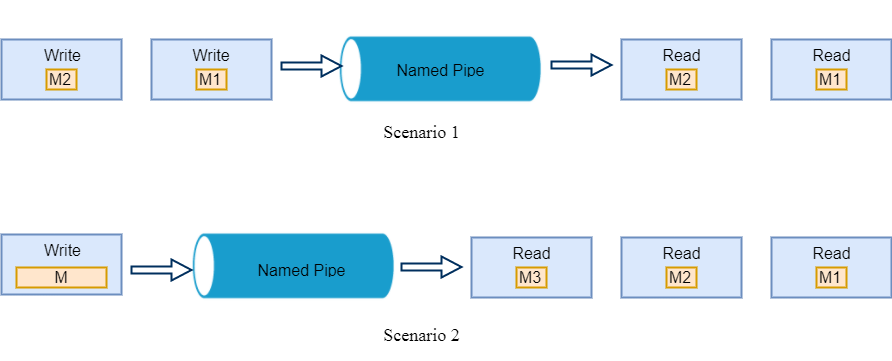
\includegraphics[scale=.415]{Figures/event}
 \caption{Break one send/multiple receive into multiple send/receive events}
\label{event}
\end{figure}

Before jumping into solving the problem we need to define what is a communication event. In this work, a communication event in the dual trace is defined as a successfully send and received message. There are four essential elements in this event: send function call, receive function call, the sent message in the sender's memory and the received message in the receiver's memory. However, in some cases, the send and receive operation are not always exactly paired. For example, the receiver buffer is small than the sender buffer, the receive function has to be called multiple times to receive one message from the sender. In this case, the one send V.S. multiple receives event is broken into multiple send V.S. receive events as shown in Figure \ref{event}. 



\section{Define the Scope}
Named pipe, MQMS, HTTP, TCP/UDP socket are targeted in this work since they are the most widely used ones in windows server/client service and are the ones used in the popular Window Communication Foundation.

\section{Obtain Background Knowledge}
In order to synchronize the messaging of both side of the traces, we need to investigate the communication methods to figure out how they looks like in the assembly level traces.
There are so many communication methods exists in the real world and they are updating everyday. We are not covering all of them at a time, but start from narrowing down our study into some widely used communication methods. The built prototype is extendable to support other cases.

In these work, we had investigated the Windows APIs for setting up these communication channels and sending/receiving messages in these communication channels. By understanding these APIs, we modeled the communication channels in the assembly traces. And Then we build our prototype tool based on these models. In addition, the user can refer to the channel models to define the concerned communication type through the user interface we provide in the prototype tool. Defined communication type is later on used for locating the communication events in the dual-trace.  

\section{Model the Channels}

\section{Build the Prototype}

\section{Verify the Model and the Prototype Tool}


\setlength{\unitlength}{\savedunitlength}
